\section{Obbiettivo}

L'obiettivo di questa esercitazione \`{e}  quello di realizzare un cluster di 2 nodi nel quale si dovrà avere \textit{Pacemaker} come Cluster Resource Manager (\textit{CRM}), \textit{Corosync} come \textit{Cluster Engine}, \textit{Apache} come \textit{Web Server} e \textit{DRBD} per creare una risorsa replicata in tutti i nodi del cluster (\textit{Distributed Replicated Storage System}).

\section{Ambiente di Lavoro}

Questa esercitazione \`{e} stata svolta all'interno del seguente ambiente di lavoro:

\begin{itemize}
	\item \textbf{Hardware}: 
		\begin{itemize}
			\item \textbf{CPU}: AMD Ryzen 9 5900x
			\item \textbf{RAM}: 32 GB DDR4 @3200 MHz
		\end{itemize}
	\item \textbf{Software}:
		\begin{itemize}
			\item \textbf{Host OS:} Arch Linux
			\item \textbf{Guest OS}: Fedora 34 Server
			\item \textbf{Virtualization Software}: VirtualBox 6.1
		\end{itemize}
\end{itemize}

\section{Configurazione Macchine}

Per questa esercitazione sono necessarie 2 macchine virtuali che saranno i due nodi del nostro cluster. Ogni macchina \`{e} stata configurata come segue:

\begin{itemize}
	\item \textbf{Cores:} 5 Core
	\item \textbf{RAM:} 5GB
	\item \textbf{Dischi di archiviazione:}
		\begin{itemize}
			\item Disco Principale da 25 GB
			\item Disco per risorsa condivisa da 1 GB
		\end{itemize}
	\item \textbf{Scheda di Rete:} Scheda di rete con Bridge
\end{itemize}

\`{E} consigliato configurare una sola macchina, installare e configurare il sistema operativo e i software necessari, per poi utilizzare la funzione 'Clona' di VirtualBox per generare una copia identica senza dover ripetere tali operazioni nuovamente. Durante la fase di clonazione della macchina \`{e} necessario selezionare l'opzione "Generare nuovi Mac Address per ogni Network Adapter" come policy per la gestione dei Mac Address.

\begin{center}
	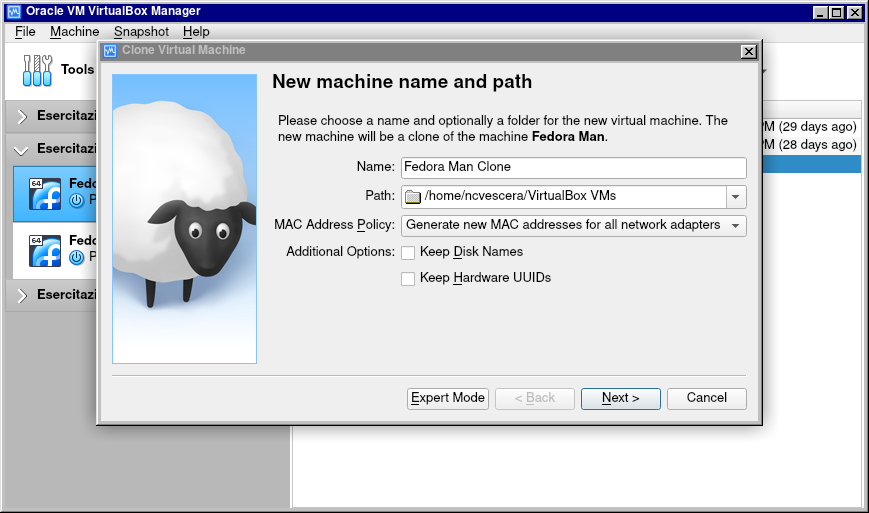
\includegraphics[scale=0.4]{screens/vb_macpolicy.png}
\end{center}
 
\section{Configurazione Software}

%% forse ci posso aggiungere una breve introduzione ...

\subsection{Sistema Operativo}

Qui ci va uno speghino un po dettagliato di come ho installato il sistema operativo. Piu immagini che altro, deve essere una brevissima guida.

Notare come di default il servizio sshd e' attivo e ho utilizzato ssh per connettermi e modificare le macchine

\subsection{Software Necessario}

Appena ho terminato la fase di installazione del SO, ho provveduto ad aggiornarlo con il seguente comando, per evitare probelmi di compatibilit\`{a} e software obsoleto:

\begin{lstlisting}[style=cmd]
 sudo dnf -y upgrade
\end{lstlisting} 
\ \\
Poi ho installato i pacchetti necessari (\textit{Pacemaker}, \textit{Corosync}, \textit{Apache} e \textit{DRBD}) con: 

\begin{lstlisting}[style=cmd]
 sudo dnf -y install pacemaker corosync pcs
 sudo dnf -y install drbd-pacemaker drbd-udev
 sudo dnf -y install httpd
 sudo dnf -y install iptables-services
\end{lstlisting} 

\subsection{IP}

Ho assegnato IP statici alle macchine per essere sicuro di poterle sempre raggiungere e che il DHCP del mio router non gli assegni indirizzi diversi col passare del tempo. Per farlo ho utilizzato i seguenti comandi:

\begin{itemize}
	\item Macchina 1: 
	\begin{lstlisting}[style=cmd]
 sudo nmcli connection modify enp0s3 IPv4.address 192.168.178.52/24
 sudo nmcli connection modify enp0s3 IPv4.gateway 192.168.178.1
 sudo nmcli connection modify enp0s3 IPv4.dns 8.8.8.8
 sudo nmcli connection modify enp0s3 IPv4.method manual
	\end{lstlisting}
	\item Macchina 2:
		\begin{lstlisting}[style=cmd]
 sudo nmcli connection modify enp0s3 IPv4.address 192.168.178.53/24
 sudo nmcli connection modify enp0s3 IPv4.gateway 192.168.178.1
 sudo nmcli connection modify enp0s3 IPv4.dns 8.8.8.8
 sudo nmcli connection modify enp0s3 IPv4.method manual
	\end{lstlisting}
\end{itemize}
\ \\
Con la prima riga di ogni set di istruzioni vado a specificare l'indirizzo IP che voglio assegnare alla macchina con tanto di subnet mask, la seconda riga indica l'indirizzo del default gateway e la terza specifica il DNS che voglio utilizzare.
\ \\
Per rendere effettive le modifiche basta riavviare il sistema (\lstinline[style=cmd]|sudo reboot|).\\
Si pu\`{o} controllare il successo di questa operazione analizzando l'output del comando
\begin{lstlisting}[style=cmd]
 route -n
\end{lstlisting}
se restituisce qualcosa vuol dire che il tutto \`{e} andato a buon fine.\\

\begin{lstlisting}[style=output]
 Kernel IP routing table
 Destination     Gateway         Genmask       ...   Iface
 0.0.0.0         192.168.178.1   0.0.0.0       ...   enp0s3
 192.168.178.0   0.0.0.0         255.255.255.0 ...   enp0s3
\end{lstlisting}
Un possibile esempio di output.
\subsection{hosts \& hostname}
\label{sec:hosts}

Ho modificato il file \lstinline[style=cmd]|/etc/hostname| definendo un nome diverso per ogni macchina in modo tale da poterle distinguere pi\`{u} facilmente durante le sessioni SSH: 

\begin{itemize}
	\item Nome Macchina 1: fedoraman
	\item Nome Macchina 2: fedoragirl
\end{itemize}
\ \\
In entrambe le macchine, alla fine del file \lstinline[style=cmd]|/etc/hosts| ho aggiunto le seguenti righe per facilitare poi la configurazione degli altri servizi:

\begin{lstlisting}[style=cmd]
 192.1168.178.52 Fedoraman
 192.1168.178.53 Fedoragirl
\end{lstlisting}

\subsection{Firewall}

Per evitare problemi di comunicazione tra le varie macchine ho deciso di disabilitare il firewall:

\begin{lstlisting}[style=cmd]
 sudo systemctl stop firewalld
 sudo systemctl disable firewalld
\end{lstlisting}

\subsection{PCSD}
\label{sec:pcsd}
\textit{le operazioni di questa sezione sono state eseguite in entrambe le macchine }\\
\ \\
Per prima cosa ho cambiato la password dell'utente \lstinline[style=cmd]|hacluster| in quanto servir\`{a} per l'autenticazione dei vari nodi in alcuni passaggi successivi:

\begin{lstlisting}[style=cmd]
 sudo passwd hacluster
\end{lstlisting}
\ \\
Successivamente ho abilitato il servizio e l'ho avviato con:

\begin{lstlisting}[style=cmd]
 sudo systemctl enable pcsd
 sudo systemctl start pcsd
\end{lstlisting}

\subsection{Corosync}

In entrambe le macchine ho provveduto alla configurazione di \lstinline[style=cmd]|corosync| andando a popolare il file \lstinline[style=cmd]|/etc/corosync/corosync.conf| con il seguente contenuto:

\begin{lstlisting}[style=cmd]
 totem {
   version: 2
   cluster_name: ExampleCluster
   transport: knet
   crypto_cipher: aes256
   crypto_hash: sha256
 }

 nodelist {
   node {
      ring0_addr: Fedoraman
      name: node1
      nodeid: 1
   }
	
   node {
      ring0_addr: Fedoragirl
      name: node2
      nodeid: 2
  }
 }

 quorum {
   provider: corosync_votequorum
   two_node: 1
 }

 logging {
   to_logfile: yes
   logfile: /var/log/cluster/corosync.log
   to_syslog: yes
   timestamp: on
 }
\end{lstlisting}
\ \\
Nella sezione \lstinline[style=cmd]|totem| ho impostato il nome del cluster modificando l'attributo \lstinline[style=cmd]|cluster_name|. La sezione \lstinline[style=cmd]|nodelist| conterr\`{a} l'elenco di tutti i nodi del cluster, per ogni nodo ho aggiunto la sottosezione \lstinline[style=cmd]|node{}| con gli attributi:

\begin{itemize}
	\item \lstinline[style=cmd]|ring0_addr|: indica l'indirizzo del nodo, nel mio caso \`{e} \lstinline[style=cmd]|Fedoraman| per via della configurazione in \autoref{sec:hosts}
	\item \lstinline[style=cmd]|name|: il nome da assegnare al nodo
	\item \lstinline[style=cmd]|nodeid|: un numero progressivo che identifica il nodo
\end{itemize}

\subsection{Autenticazione dei Nodi}

In ogni macchina ho effettuato l'autenticazione del nodo al cluster con i seguenti comandi:

\begin{lstlisting}[style=cmd]
 sudo pcs client local-auth -u hacluster
 sudo pcs cluster auth -u hacluster
\end{lstlisting}
\ \\
La password da utilzzare in questa fase \`{e} quella dell'utente \lstinline[style=cmd]|hacluster| scelta al punto \autoref{sec:pcsd}

\subsection{Avvio Cluster}

Configuro l'avvio automatico del cluster e lo faccio partire con i seguenti comandi:

\begin{lstlisting}[style=cmd]
 sudo pcs cluster setup ExampleCluster node1 node2 --force
 sudo pcs cluster start --all
 sudo pcs cluster enable --all
\end{lstlisting}
\ \\
Questa operazione deve essere eseguita in una sola macchina, non importa quale, io per comodit\`{a} eseguir\`{o} sempre questo tipo di operazioni in \lstinline[style=cmd]|Fedoraman(node1)|.
\ \\
Controllo il corretto funzionamento del cluster tramite il comando:

\begin{lstlisting}[style=cmd]
 sudo pcs status
\end{lstlisting}
\ \\
Se ho un output come il seguente vuol dire che il tutto \`{e} andato a buon fine (\`{e} importante che i nodi risultino \lstinline[style=cmd]|Online|):

\begin{lstlisting}[style=output]
 Cluster name: ExampleCluster
 
 WARNINGS:
 No stonith devices and stonith-enabled is not false
 
 Cluster Summary:
    * Stack: corosync
    * Current DC: node1 (version 2.1.1-9.fc34-77db578727) - partition with quorum
    * Last updated: Wed Nov  3 18:17:32 2021
    * Last change:  Wed Nov  3 18:02:47 2021 by hacluster via crmd on node1
    * 2 nodes configured
    * 0 resource instances configured
 
 Node List:
    * Online: [ node1 node2 ]
 
 Full List of Resources:
    * No resources
 
 Daemon Status:
    corosync: active/enabled
    pacemaker: active/enabled
    pcsd: active/enabled
\end{lstlisting}

\subsection{Cluster Property}

Ho disabilitato le property \lstinline[style=cmd]|stonith| e \lstinline[style=cmd]|quorum| in quanto la prima non \`{e} necessaria ai fini di questa esercitazione e la seconda dato che non ho un numero sufficiente di macchine per utilizzare questa propriet\`{a} (ne servono minimo 3).

\begin{lstlisting}[style=cmd]
 sudo pcs property set stonith-enabled=false
 sudo pcs property set no-quorum-policy=ignore
\end{lstlisting}

\subsection{Cluster IP}

Assegno un IP al cluster in modo tale da raggiungere il server web, che verr\`{a} configurato in seguito, e altri possibili servizi:

\begin{lstlisting}[style=cmd]
 sudo pcs resource create floating_ip ocf:heartbeat:IPaddr2 ip=192.168.178.55 cidr_netmask=24 op monitor interval=60s
\end{lstlisting}
\ \\
L'indirizzo viene specificato con il parametro \lstinline[style=cmd]|ip=| e la subnet mask con \lstinline[style=cmd]|cidr_netmask=|. \`{E} importante notare che l'IP scelto deve appartenere alla stessa rete delle macchine e non deve essere utilizzato da nessun altro dispositivo !

\subsection{Risorsa HTTP}

Aggiungo la risorsa HTTP al cluster in modo tale da avere un server web sempre attivo anche se il nodo principale cade:

\begin{lstlisting}[style=cmd]
 sudo pcs resource create http_server ocf:heartbeat:apache configfile="/etc/httpd/conf/httpd.conf" op monitor timeout="20s" interval="60s"
\end{lstlisting}

\subsection{Partizionamento Disco Condiviso}
\label{sec:partizione}

Procedo al partizionamento del secondo disco presente in tutte e due le macchine, con il seguente comando posso controllare il suo nome (di solito \`{e} \lstinline[style=cmd]|/dev/sdb|):

\begin{lstlisting}[style=cmd]
 sudo fdisk -l
\end{lstlisting}
\ \\
Partiziono effettivamente il disco con:

\begin{lstlisting}[style=cmd]
 sudo fdisk /dev/sdb
\end{lstlisting}
\ \\
Si aprir\`{a} un menu interattivo e dovr\`{o} digirare i seguenti comandi:

\begin{itemize}
	\item \lstinline[style=cmd]|n|: nuova partizione
	\item \lstinline[style=cmd]|p|: partizione primaria
	\item \lstinline[style=cmd]|1|: numero di partizioni
	\item \lstinline[style=cmd]|ENTER|: primo settore (utilizzare il valore di default)
	\item \lstinline[style=cmd]|ENTER|: ultimo settore (utilizzare il valore di default)
	\item \lstinline[style=cmd]|w|: scrive le modifiche
	\item \lstinline[style=cmd]|q|: esce dal programma
\end{itemize}
\ \\
Oppure posso effettuare il tutto in maniera autoamtica con:

\begin{lstlisting}[style=cmd]
 sed -e 's/\s*\([\+0-9a-zA-Z]*\).*/\1/' << EOF | fdisk /dev/sdb
    n # new partition
    p # primary partition
    1 # partition number 1
      # default - start at beginning of disk 
      # default - stop at ending of disk 
    w # write the partition table
    q # and we're done
 EOF
\end{lstlisting}

\subsection{Configurazione DRBD}

Prima di tutto, devo andare a modificare la policy di sicurezza di SELinux per DRBD, dato che ne impedisce (di defualt) il corretto funzionamento, tramite il seguetne comando:

\begin{lstlisting}[style=cmd]
 sudo semanage permissive -a drbd_t
\end{lstlisting}
\ \\
Fatto ci\`{o}, posso andare a configurare DRBD popolando il file di configurazione \lstinline[style=cmd]|/etc/drbd.d/wwwdata.res| con il seguente contenuto:

\begin{lstlisting}[style=cmd]
 resource wwwdata {
    protocol C;
    device /dev/drbd0;

    syncer{
        verify-alg sha1;
    }

    net {
        cram-hmac-alg sha1;
        shared-secret "barisoni";
    }


    on fedoraman {
        disk /dev/sdb1;
        address 192.168.178.52:7788;
        meta-disk internal;
    }
    on fedoragirl {
        disk /dev/sdb1;
        address 192.168.178.53:7788;
        meta-disk internal;
    }
 }
\end{lstlisting}
\ \\
Ho scelto una chiave per l'algoritmo di crittografia tramite la propriet\`{a} \lstinline[style=cmd]|shared-secret|. \`{E} importante notare che \lstinline[style=cmd]|on fedoraman| e \lstinline[style=cmd]|on fedoragirl| sono i nomi che ho impostato nel punto \autoref{sec:hosts} e nelle relative sezioni ho specificato il nome del disco da utilizzare (sar\`{a} sempre \lstinline[style=cmd]|/dev/sdb1| per via della configurazione in \autoref{sec:partizione}), l'indirizzo IP della macchina (non sembra possibile utilizzare gli alias definiti in \autoref{sec:hosts}) e una porta a scelta per la comunicazione (ho utilizzato la \lstinline[style=cmd]|7788|)\ \\
\ \\
Creo dunque la risorsa drbd:

\begin{lstlisting}[style=cmd]
 sudo drbdadm create-md wwwdata
\end{lstlisting}
\ \\
Abilito il modulo kernel per rendere sempre utilizzabile la risorsa, anche ai prossimi riavvii:

\begin{lstlisting}[style=cmd]
 sudo modprobe drbd
 sudo echo "drbd" >> /etc/modules-load.d/drbd.conf
\end{lstlisting}
\ \\
Completo la configurazione della risorsa con:

\begin{lstlisting}[style=cmd]
 sudo drbdadm up wwwdata
 sudo drbdadm -- --overwrite-data-of-peer primary all
 
 sudo drbdadm primary --force wwwdata
\end{lstlisting}
\ \\
Il terzo comando deve essere eseguito solo sulla prima macchina !\\
Per monitorare l'avanzamento del processo ho utilizzato il seguente comando: \lstinline[style=cmd]|watch cat /proc/drbd|.\\
\ \\
Infine la abilito per far si che si avvii in automatico:

\begin{lstlisting}[style=cmd]
 sudo systemctl enable drbd
 sudo systemctl start drbd
\end{lstlisting}

\subsection{Formattazione Risorsa DRBD}

Procedo con la formattazione della risorsa drbd creata in precedenza e con l'aggiunta di una pagina web per controllare il corretto funzionamento:

\begin{lstlisting}[style=cmd]
 mkfs.xfs /dev/drbd0
 sudo mount /dev/drbd0 /mnt
 sudo echo "<h1>Hello World</h1>" >> /mnt/index.html
 sudo umount /dev/drbd0
\end{lstlisting}

\subsection{Risorsa DRBD}

Aggiungo al cluster la risorsa DRBD creata in precedenza:

\begin{lstlisting}[style=cmd]
 sudo pcs cluster cib drbd_cfg
 sudo pcs -f drbd_cfg resource create WebData ocf:linbit:drbd drbd_resource=wwwdata op monitor interval=60s
 sudo pcs -f drbd_cfg resource promotable WebData promoted-max=1 promoted-node-max=1 clone-max=2 clone-node-max=1 notify=true
 sudo pcs cluster cib-push drbd_cfg --config
\end{lstlisting}
\ \\
Controllo il risultato di questa operazione con il comando:

\begin{lstlisting}[style=cmd]
 sudo pcs status
\end{lstlisting}
\ \\
Mi aspetto un outpit simile al seguente:

\begin{lstlisting}[style=output]
 Cluster name: ExampleCluster
 Cluster Summary:
    * Stack: corosync
    * Current DC: node1 (version 2.1.1-9.fc34-77db578727) - partition with quorum
    * Last updated: Tue Dec 14 10:39:46 2021
    * Last change:  Mon Nov  8 10:35:32 2021 by root via cibadmin on node1
    * 2 nodes configured
    * 5 resource instances configured

Node List:
    * Online: [ node1 node2 ]

Full List of Resources:
    * Resource Group: Fedora_group:
        * floating_ip	(ocf::heartbeat:IPaddr2):	 Started node1
        * http_server	(ocf::heartbeat:apache):	 Started node1
    * Clone Set: WebData-clone [WebData] (promotable):
        * Masters: [ node1 ]
        * Slaves: [ node2 ]

Daemon Status:
corosync: active/enabled
pacemaker: active/enabled
pcsd: active/enabled

\end{lstlisting}
%%incollare outpt con tutte le risorse pronte

\subsection{Risorsa WebFS}

Per ultimo aggiungo al cluster la risorsa WebFS per far si che i dati del Web Server siano replicati in tutti i nodi:

\begin{lstlisting}[style=cmd]
 sudo pcs cluster cib fs_cfg
 sudo pcs -f fs_cfg resource create WebFS Filesystem device="/dev/drbd0" directory="/var/www/html" fstype="xfs"
 sudo pcs -f fs_cfg constraint colocation add WebFS with WebData-clone INFINITY with-rsc-role=Master
 sudo pcs -f fs_cfg constraint order promote WebData-clone then start WebFS
 sudo pcs -f fs_cfg constraint colocation add http_server with WebFS INFINITY
 sudo pcs -f fs_cfg constraint order WebFS then http_server
 sudo pcs cluster cib-push fs_cfg --config
\end{lstlisting}
\ \\
Nei comandi dove compare la clausula \lstinline[style=cmd]|order| vado a specificare l'ordine con cui le risorse devono essere avviate, per esempio con \lstinline[style=cmd]|order WebFS then http_server| sto dicendo al cluster di avviare prima la risorsa WebFs e poi il server web.

\subsection{Failover Test}

Come test finale ho simulato un failover del nodo principale con il seguente comando:

\begin{lstlisting}[style=cmd]
 sudo pcs node standby node1
\end{lstlisting}
\ \\
Controllo quindi che \lstinline[style=cmd]|node2| venga promosso a master e si avvii la risorsa WebFs:

\begin{lstlisting}[style=cmd]
 sudo pcs status
\end{lstlisting}

\begin{lstlisting}[style=output]
 Cluster name: ExampleCluster
 Cluster Summary:
    * Stack: corosync
    * Current DC: node1 (version 2.1.1-9.fc34-77db578727) - partition with quorum
    * Last updated: Tue Dec 14 10:53:27 2021
    * Last change:  Tue Dec 14 10:53:10 2021 by root via cibadmin on node1
    * 2 nodes configured
    * 5 resource instances configured

 Node List:
    * Node node1: standby
    * Online: [ node2 ]

 Full List of Resources:
    * Resource Group: Fedora_group:
        * floating_ip	(ocf::heartbeat:IPaddr2):	 Started node2
        * http_server	(ocf::heartbeat:apache):	 Started node2
    * Clone Set: WebData-clone [WebData] (promotable):
        * Masters: [ node2 ]
        * Stopped: [ node1 ]
    * WebFS	(ocf::heartbeat:Filesystem):	 Started node2

 Daemon Status:
 corosync: active/enabled
 pacemaker: active/enabled
 pcsd: active/enabled
\end{lstlisting}
\ \\
Una volta assicurato il successo di questa operazione riporto in vita il \lstinline[style=cmd]|nodo1| con:

\begin{lstlisting}[style=cmd]
 sudo pcs node unstandby node1
\end{lstlisting}